\documentclass[12pt,a4paper]{article}

% ----------------------------
% Packages
% ----------------------------
\usepackage[utf8]{inputenc}
\usepackage[T1]{fontenc}
\usepackage{lmodern}
\usepackage{geometry}
\usepackage{setspace}
\usepackage{graphicx}
\usepackage{float}
\usepackage{amsmath, amssymb}
\usepackage{hyperref}
\usepackage{booktabs}
\usepackage{listings}
\usepackage{xcolor}
\usepackage{caption}
\usepackage{subcaption}
\usepackage{fancyhdr}
\usepackage{forest}

% Compact unnumbered heading for small intra-section labels.
\newcommand{\minorheading}[1]{%
    \vspace{0.75em}%
    \noindent\textbf{#1}\par
    \vspace{0.25em}%
}
\setcounter{secnumdepth}{3}
\setcounter{tocdepth}{3}


% ----------------------------
% Page Setup
% ----------------------------
\geometry{margin=1in}
\onehalfspacing
\pagestyle{fancy}
\fancyhf{}
\fancyhead[L]{Project Diary: Public Transport Oldenburg}
\fancyhead[R]{\thepage}

% ----------------------------
% Code Listings Setup
% ----------------------------
\lstset{
    basicstyle=\ttfamily\small,
    keywordstyle=\color{blue},
    commentstyle=\color{gray},
    stringstyle=\color{red},
    numbers=left,
    numberstyle=\tiny,
    breaklines=true,
    frame=single
}

% ----------------------------
% Document Info
% ----------------------------
\title{\textbf{Improving the Usability of Public Transport in Oldenburg}\\
\vspace{0.5cm}
\large Project Diary}
\author{
    \textbf{Authors:} Maik Bernert, Robin Harlammert, Linus Müller-Holthusen \\
    \textbf{Supervisor:} Pavel Karpashevich \\
    \texttt{pavel.karpashevich@uni-oldenburg.de}
}
\date{\today}

% ----------------------------
% Document Start
% ----------------------------
\begin{document}

\maketitle
\newpage
\pagenumbering{roman}

\tableofcontents
\listoffigures
\listoftables
\newpage
\pagenumbering{arabic}

% ----------------------------
% Chapter 1: Introduction
% ----------------------------
\section{Introduction}
\subsection{Background and Motivation}
Public transport in Oldenburg is used by both established residents and newcomers. While the system is fully operational, its accessibility and usability may vary depending on users’ familiarity with the city and its transport infrastructure. In this context, newcomers represent a particularly relevant user group, as their experiences can reveal initial barriers that may be less visible to long-term residents. Although established residents may also encounter challenges, this project specifically focuses on the perspective of newcomers. Its aim is to examine their experiences with public transport in Oldenburg and to propose and implement digital measures for improving the overall user experience for this target group.

\subsection{Problem Statement}
This project aims to support newcomers in Oldenburg by improving their experience with public transport. In this context, the term “newcomer” refers to people who are new to Oldenburg, whether they have moved from another region, city, or country or just visit the city. To establish a clear baseline for this target group, we define newcomers as people who have lived/stayed in Oldenburg for less than two years. Newcomers to Oldenburg may face challenges in the following areas:

\begin{itemize}
    \item Finding the right connection
    \item Navigating/Routing
    \item Buying and choosing tickets
    \item Understanding fares and validity
    \item Payments
    \item Knowing which app to use
    \item Language
    \item Real-time information
\end{itemize}

This information is evidenced by both, literature (\cite{usability},\cite{DZIEKAN2007489},\cite{mindthegap}) and the group's personal experience.

\subsection{Objectives}
This project will follow the Interaction Design Cycle visible in \autoref{fig:interaction-design-cycle} as presented in the lecture.

\begin{figure}[h!]
    \centering
    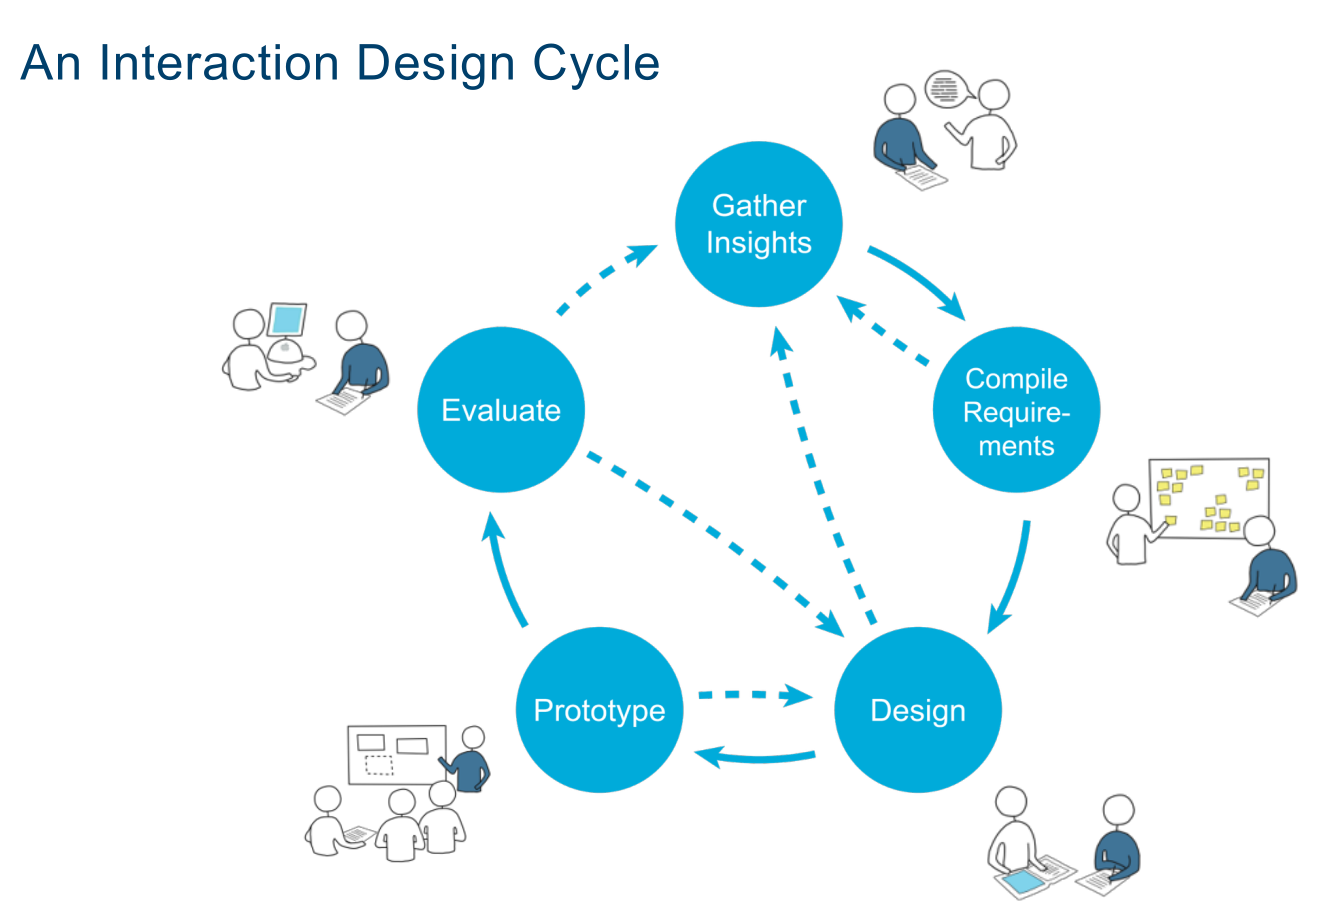
\includegraphics[width=1\linewidth]{interaction_design_cycle.png}
    \caption{Interaction Design Cycle as presented in the lecture.}
    \label{fig:interaction-design-cycle}
\end{figure}

For each of these steps, our higher-level objectives consist of the following:
\begin{enumerate}
    \item \textbf{Gather Insights:} Gather real-life information of what issues people have in public transport and identify which of them especially apply to newcomers.
    \item \textbf{Compile Requirements:} Distill the previous findings into concrete requirements describing the system to be implemented later on.
    \item \textbf{Design:} Create an application-prototype mockup that visually fullfills the compiled requirements.
    \item \textbf{Prototype:} Create a prototype the fullfills the requirements and implements the visual design of the design.
    \item \textbf{Evaluate:} Gather and evaluate feedback from real users and their interaction with the prototype.
\end{enumerate}


\section{Gathering Insights}
\subsection{Methodology}
To understand the genuine needs and pain points of public transport users, we focused mainly on inquiries and initially designed an interview sheet which we shortly after adjusted such that it doubles down as a survey sheet. This sheet is visible in the appendix as \autoref{fig:inteviewsheet}. The sheet way mainly designed to enable quick interviews for people at bus stops as they will likely be on a schedule to catch a bus. With this in mind, the red line in the sheet goes from an about you section straight to public transport use and people's main difficulties. It also asks for used apps so we can identify which routing apps are the most popular and openly asks for improvements. As visible in the document, there are free text fields which were useful to avoid the interviewer effect as people could freely answer those questions. The main segment of the sheet was the third part (main difficulties).

As we had previously done literature research on known issues in public transport in general, we also extended our literature research, thus also referring to existing knowledge. Thus, we used to following methods for gathering insights as presented in the lecture:

\begin{center}
\begin{forest}
for tree={
    draw,
    rounded corners,
    align=center,
    edge={-},
    parent anchor=south,
    child anchor=north,
    l sep=12pt,
    s sep=10pt
}
[Gathering Insights
    [Inquiries
        [Interview]
        [Survey]
    ]
    [Existing Knowledge
        [Literature Review]
    ]
]
\end{forest}
\end{center}



From our inquiries, we collected 54 responses in total. A significant portion of these, comprising 38 responses, came from people whom we consider newcomers. An initial problem that arised within the survey was sampling bias. As the survey was distributed exclusively among private contacts whose newcomer status was known in advance, the resulting sample was skewed toward younger age groups and people from Germany. Another effort driver was analyzing the free-text fields as some people in the surveys would give their answers in german. And some answers were rather hard to understand.

\subsection{Interpretation}
\subsubsection{Evaluation of Free-Text Responses}
The free-text responses were evaluated qualitatively and used to complement the predefined survey categories. Responses that described concrete needs, suggestions, or recurring problems were considered as direct input for prototype development. For example, specific remarks about missing information, confusing ticket options, or accessibility-related issues were translated into potential design requirements. Responses that did not introduce a clearly new aspect were assigned to one of the existing problem categories in order to keep the analysis consistent with the structured survey data. This approach allowed us to preserve individual user perspectives while still maintaining comparability across all survey responses.

\subsubsection{Visualizing Results}
We developed automated scripts to analyze the survey responses. These scripts cross-referenced various data points, such as the relationship between a user's residence duration and their understanding of the system, as well as age versus usage frequency. 


We automatically generated a comprehensive set of graphs and charts to visually communicate our findings. Key visualizations highlight primary pain points; for instance, \autoref{fig:group_problems} clearly illustrates the specific hurdles newcomers encounter most often.

\begin{figure}[h!]
    \centering
    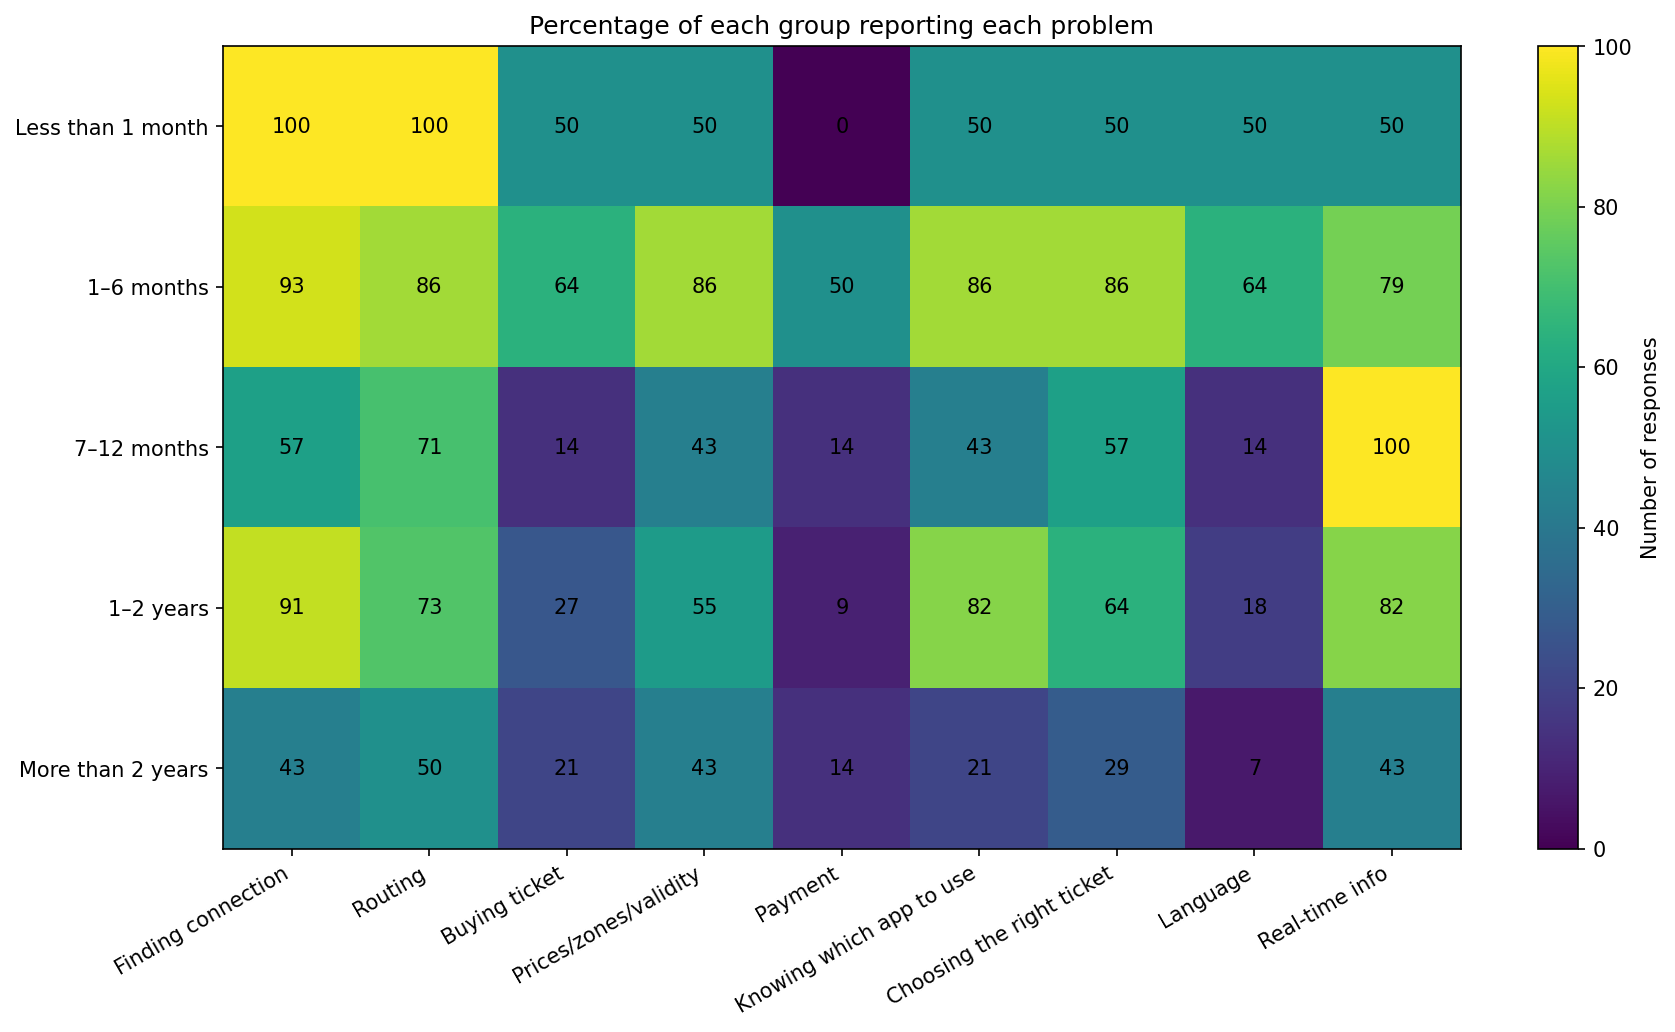
\includegraphics[width=1.0\linewidth]{graph_comparison.png}
    \caption{Matrix heatmap showing the percentage of respondents per occurring public transport issue by length of stay in Oldenburg.}
    \label{fig:group_problems}
\end{figure}


\section{Compiling Requirements}
\subsection{Scope Definition}
The scope of this project is intentionally limited because the objective is not to develop a complete market-ready mobility product. Instead, the project focuses on the human-computer interaction aspects of public transport use, especially how newcomers understand routes, tickets, and transport-related information. Due to the limited project timeframe, the prototype prioritizes interaction design, usability, and the communication of relevant information over complete technical coverage of all mobility scenarios. Consequently, several features are simplified or represented conceptually, as the main purpose of the prototype is to evaluate whether the proposed interface can reduce confusion and support users in making better transport decisions.

The scope of this project is limited to a prototype for supporting public transport use within Oldenburg. Therefore, rides outside of Oldenburg are not shown, as the main objective is to address the needs of newcomers using public transport in the local urban context. In addition, the available bus and train data is restricted by the VBN network, which further defines the geographical and technical boundaries of the prototype.

The prototype focuses on route guidance and basic ticket-related support rather than implementing a complete transport booking or pricing system. Train pricing is therefore represented only by dummy data, since exact train prices are not central to the evaluated concept. Similarly, different ticket types are not handled separately in detail. Instead, the system primarily indicates whether bus rides are free for the user based on the available ticket information.

Some user preferences are included in the interface but are not yet connected to the routing logic. For example, bicycle and dog options are displayed as part of the user profile and route preferences, but they do not change the resulting route suggestions in the current prototype. This allows the interface concept to reflect relevant user needs while keeping the technical implementation manageable.

Furthermore, the prototype does not implement an independent routing engine. Route suggestions are based on available API data and simplified assumptions rather than on fully custom routing calculations. Taxi and car routing are also not implemented, as the project focuses specifically on public transport guidance. As a result, the prototype should be understood as a focused interaction and usability prototype rather than a complete replacement for existing mobility platforms.


\subsection{Requirements}
By combining the major issues we gathered with the prototipical scope 


\subsubsection{Functional Requirements}

\begin{table}[h]
\centering
\begin{tabular}{|p{2cm}|p{12cm}|}
\hline
\textbf{ID} & \textbf{Requirement} \\
\hline
FR1 & The system shall provide public transport route planning for Oldenburg, Germany. \\
\hline
FR2 & The system shall allow users to search routes between a start location and a destination and display route details such as transport type (Taxi, Bus, Train), stops, transfers, duration, departure time, and arrival time. \\
\hline
FR3 & The system shall integrate the HAFAS Public Transport endpoint to retrieve public transport connection and departure data where available. \\
\hline
FR4 & The system shall provide an onboarding process for creating a user profile, including available tickets, preferred transport modes, disabilities or accessibility needs, walking distance preferences, and regular travel habits. \\
\hline
FR5 & The system shall personalize route and ticket information based on the user profile, including a compact ticket overview with validity information and basic route suitability guidance. \\
\hline
\end{tabular}
\caption{Functional Requirements}
\label{tab:functional-requirements}
\end{table}

\subsubsection{Non-Functional Requirements}

\begin{table}[h]
\centering
\begin{tabular}{|p{2cm}|p{12cm}|}
\hline
\textbf{ID} & \textbf{Requirement} \\
\hline
NFR1 & The system shall be simple, beginner-friendly, and easy to understand for users with little public transport experience. \\
\hline
NFR2 & The system shall present ticket, route, stop, and departure information in a compact and understandable way. \\
\hline
NFR3 & The system shall be mobile-friendly, responsive, and usable as an installable Progressive Web App. \\
\hline
NFR4 & The system shall keep route, ticket, and departure information as up-to-date as possible within the limitations of the available HAFAS data source. \\
\hline
NFR5 & The system shall provide trustworthy and accessible guidance by using clear labels, readable text, sufficient contrast, fallback messages for missing data, and transparent ticket or route information. \\
\hline
\end{tabular}
\caption{Non-Functional Requirements}
\label{tab:non-functional-requirements}
\end{table}


\section{Designing}
\subsection{Design Evaluation and Requirement Mapping}

To visualize the user experience and ensure alignment with the project goals, a low-fidelity prototype was created using Figma. The primary objective of this mockup phase was to conceptualize a user interface that feels intuitive, particularly for users unfamiliar with complex public transport tariff systems.

By mapping the mockups against the established Functional Requirements (FR) and Non-Functional Requirements (NFR), it is possible to evaluate which goals have been structurally addressed during the design phase and which are delegated to backend implementation.

\subsubsection{Functional Requirements Check}

The current Figma prototypes focus primarily on the ticket optimization flow rather than on complete routing mechanics.

\minorheading{Addressed in Design}

\begin{itemize}
    \item \textbf{FR1 (Route Planning for Oldenburg):}  
    The start screen establishes the geographical and contextual scope of Oldenburg, for example by presenting journeys such as \emph{Hauptbahnhof to Stadtmuseum} within \emph{Zone Oldenburg I}.

    \item \textbf{FR5 (Personalized Ticket Overview):}  
    This requirement is strongly fulfilled in the design. An automated verification step (e.g., ``Automatic check running \dots'') combined with a step-by-step wizard collects relevant traveler information such as age, bicycles, dogs, and travel intent (single trip versus commuting). Based on this input, the system generates a highly compact and personalized ticket recommendation displayed on the final screen.
\end{itemize}

\minorheading{Missing or Delegated to Implementation}

\begin{itemize}
    \item \textbf{FR2 (Route Details):}  
    The current screens do not display a detailed route breakdown, such as intermediate stops, transfers, or transport modes. This functionality will need to be designed separately or integrated alongside the ticket view.

    \item \textbf{FR4 (Onboarding/Profile):}  
    Although the UI references an ``Existing pass check,'' the complete onboarding or profile creation flow-where users initially provide this information-is not shown in the current mockups.

    \item \textbf{FR3 (HAFAS API Integration):}  
    As the prototype is static, live API integration cannot be visually demonstrated at this stage.
\end{itemize}

\subsubsection{Non-Functional Requirements Check}

The design decisions strongly emphasize usability, accessibility, and clarity.

\minorheading{Addressed in Design}

\begin{itemize}
    \item \textbf{NFR1 (Simple and Beginner-Friendly):}  
    The wizard-based interaction breaks down complex tariff systems into a sequence of simple questions such as ``Who is travelling?'' and ``What should we optimise?''. The reassurance text (``We'll only ask what changes the price'') further reduces cognitive load for first-time users.

    \item \textbf{NFR2 (Compact Information):}  
    The final ticket overview is highly scannable, highlighting price, validity, and zone information using clear visual cards. The optimized recommendation (e.g., a 4x Ticket) is explicitly compared against a standard Single Ticket.

    \item \textbf{NFR3 (Mobile-Friendly):}  
    The prototype is designed within a mobile viewport, featuring large touch targets, bottom-anchored primary action buttons (``Continue'', ``Buy ticket''), and vertical scrolling, making it well suited for a Progressive Web App (PWA).

    \item \textbf{NFR5 (Trustworthy and Transparent):}  
    Transparency is achieved by clearly explaining ticket recommendations, presenting price comparisons, and using standard high-contrast color schemes (blue and white) to ensure readability and user trust.
\end{itemize}

\minorheading{Delegated to Implementation}

\begin{itemize}
    \item \textbf{NFR4 (Up-to-date Data):}  
    Ensuring that departure times and ticket data remain current depends on backend systems and external data sources. This requirement cannot be validated within a static Figma prototype.
\end{itemize}

\subsubsection{Limitations of the Mockup}

Due to the static nature of Figma prototypes, certain system behaviors are only simulated. Live data retrieval from the HAFAS system (FR3, NFR4) and real-time logic based on user profiles cannot be executed. Features such as the ``Automatic check running'' indicator represent optimistic UI placeholders for backend processes. Consequently, the technical feasibility and performance of dynamic routing and optimization features will only be fully validated during the implementation and development phase.


\section{Prototyping}
\subsection{Technologies}
After gathering insights, compiling requirements, and creating the visual design, we implemented an interactive prototype. The goal was not to build a production-ready public transport app, but to make the central concept testable: users should be able to search a route, understand the connection, and receive ticket or fare guidance.

The prototype was implemented as a React and Vite web application. Tailwind CSS was used for styling, Leaflet for map display, and the VBN/HAFAS endpoint for public transport data. Profile and session data are stored locally in the browser using IndexedDB. The application state is managed centrally in a React context, which stores the selected route, trip data, profile settings, passengers, search results, and ticket-flow answers.

This technology stack was used, as it gave us the required features to fulfill the set requirements, whilst enabling us to create a PWA.

The code is separated into screen components and domain modules. Screen components are responsible for rendering the user interface and handling user interaction, while domain modules contain the underlying application logic. This structure was chosen to keep the visual implementation clearly separated from transport-specific calculations and decision rules. As a result, the code remains easier to understand, maintain, and extend, since changes to the interface do not directly affect the core logic.

Important functionality such as passenger validation, fare handling, taxi fare calculation, ticket optimization, geometry handling, and HAFAS product classification is therefore implemented outside the visual components. This also makes the corresponding logic easier to test independently from the user interface. Some of these modules are covered by automated tests, especially taxi fares, fare calculation, passenger validation, geometry, and HAFAS mode parsing. The tests help ensure that central calculations and classifications remain stable when the prototype is modified.

\subsection{Implemented Features}
The prototype covers the main user journey. Users can search for a connection, inspect route details, and continue to a ticket recommendation or taxi fare estimate. The route result list displays departure and arrival times, duration, transport lines, transfers, and walking information. The journey detail screen shows a map, timeline, boarding and exit information, and a direction indicator.

A central feature is the user profile. During onboarding, users can define whether they travel as an adult or child, which tickets they already own, which transport modes they prefer, and whether accessibility support is relevant. The profile can be enabled or disabled in the profile menu. When enabled, it filters route results and influences ticket recommendations.

The profile also contains the options ``prefer low-floor vehicles'' and ``notify driver''. These were derived from survey responses about accessibility, insecurity at stops, and the wish for better assistance. They were included as a new concept that is not directly available in DB Navigator. In the current prototype, however, these options are only represented in the interface and do not yet trigger real transport-network functionality.

The prototype also includes taxi support. If taxis are enabled in the profile, a taxi option is shown at the top of the result list. Selecting it skips the public transport ticket questions and directly shows a taxi fare estimate. The estimate uses the local Oldenburg taxi tariff with separate day and night/Sunday rates.

\subsection{Prototype Workflow}
The workflow starts with onboarding. After the profile has been created, the user enters a start and destination, selects a departure time, and searches for connections. Public transport connections lead to the journey detail screen and then to the ticket flow. The ticket flow asks only trip-relevant questions and finally shows a recommendation. Taxi connections use a shorter path and directly lead to the fare estimate because ticket rules do not apply.

\subsection{Implementation Decisions}
Several implementation decisions were made to keep the interface simple. Instead of adding many visible filters to the route planner, mode preferences are managed in the profile. This keeps the search screen less crowded while still allowing personalization. Details are also separated from the result cards: the cards show only the most important information, while the journey detail screen contains the full explanation.

For map display, the prototype uses available journey geometry where possible. If detailed geometry is missing, it falls back to simplified or estimated geometry. This supports visual understanding, but avoids implementing a complete independent routing engine.

\subsection{Requirements Checking}
The prototype fulfils the main functional requirements within the defined scope. It provides route planning for Oldenburg and surrounding VBN connections, displays relevant journey details, integrates with the HAFAS endpoint, supports a persistent user profile, and provides personalized route and ticket information. It also addresses the non-functional requirements by presenting information in a compact, mobile-friendly, and beginner-oriented interface.

However, the requirements are fulfilled at prototype level rather than production level. The route planner works with available API data, but it does not replace a full routing engine. Ticket logic is implemented as a simplified model that is sufficient for testing the concept, but it is not a legally binding fare system. Similarly, profile-based personalization is implemented for visible filtering and recommendation logic, but not for all real-world operational effects.

\section{Technical Limitations}

The prototype has several technical limitations that result from the available data sources, the project scope, and the focus on interaction design rather than full product implementation. Ticket purchasing is not supported within the prototype. Implementing this feature would require a technical and legal collaboration with official ticket providers, including access to payment systems, fare validation, and ticket issuing infrastructure. Therefore, the prototype only provides ticket-related guidance instead of enabling actual purchases.

Ticket prices are static and are not updated automatically. Since the prototype is not connected to an official fare database, prices may become outdated and should be understood as illustrative information rather than legally binding fare data. This limitation is acceptable for the purpose of evaluating whether users understand ticket recommendations and price-related information.

Accessibility-related features are also partly conceptual. Notifying bus drivers about wheelchair users is included as an idea, but it has no technical functionality in the prototype. Similarly, the options ``prefer low-floor vehicles'' and ``notify driver'' were derived from the survey results and added as design concepts. However, they currently do not affect the routing logic, since comparable functionality is not provided by DB Navigator or by the available transport data. These features therefore demonstrate a potential improvement rather than a fully implemented service.

Routing is partly estimated rather than fully exact, because the prototype relies on the available API data instead of implementing an independent routing engine. As a result, route suggestions depend on the quality and completeness of the external data source. This keeps the implementation feasible within the project while still allowing the prototype to evaluate the usability of route presentation and decision support.


\section{Evaluation}
% TODO: Add evaluation methodology and conclusion.
\subsection{Evaluation Method}
To evaluate the prototype's usability, we conducted a systematic user study utilizing the System Usability Scale (SUS). The SUS provides a high-level view of subjective usability through a simple 10-item Likert scale. It effectively measures effectiveness, efficiency, and satisfaction, ultimately yielding a single score from 0 to 100 while being very easy to administer.

We explicitly decided against the User Experience Questionnaire (UEQ) for this evaluation. While the UEQ comprehensively assesses broader dimensions, such as attractiveness, stimulation, and novelty, across 26 semantic differential items, its scope extends beyond our goals. Because our prototype primarily aims to resolve functional barriers for newcomers rather than evoke specific emotional responses or aesthetic impressions, the focused 10-item SUS offered a more direct and participant-friendly measurement of core usability.

For the administration of the study, we created an anonymous online survey using Google Forms titled ``Oldenburg Public Transport App - Usability Study'' (the full questionnaire is available for reference in \autoref{fig:googleFormsSheet}). The survey was structured into four main sections:

\begin{itemize}
    \item \textbf{About you:} This section gathered demographic data, such as age and time lived in Oldenburg, along with public transport usage habits, including frequency, purpose, and currently used apps.
    \item \textbf{Try the app:} Participants were instructed to open the prototype in a separate browser tab and complete three specific scenarios designed to mimic real situations newcomers often face.
    \begin{itemize}
        \item \textbf{Task A} involved planning a one-way weekday trip from Oldenburg Hauptbahnhof (Hbf) to Lappan (city centre).
        \item \textbf{Task B} required the user to read the app's ticket suggestion for the previous connection and pick the ticket they would actually buy.
        \item \textbf{Task C} asked users to adjust their profile to simulate using a four-ride ticket (Vierer-Ticket) and verify that the ticket counter decreased correctly.
    \end{itemize}
    After each task, users rated whether they were able to complete it and how easy it was to perform.
    \item \textbf{System Usability Scale (SUS):} Participants rated ten standard SUS statements regarding their confidence, the app's complexity, consistency, and integration of functions on a scale from 1 to 5.
    \item \textbf{Final Thoughts:} The survey concluded with open-ended questions allowing users to describe what worked well and what needed improvement, as well as whether they would use the app in real life for their public transport trips in Oldenburg.
\end{itemize}

\subsection{Discussion of Results}

\begin{figure}[h!]
    \centering
    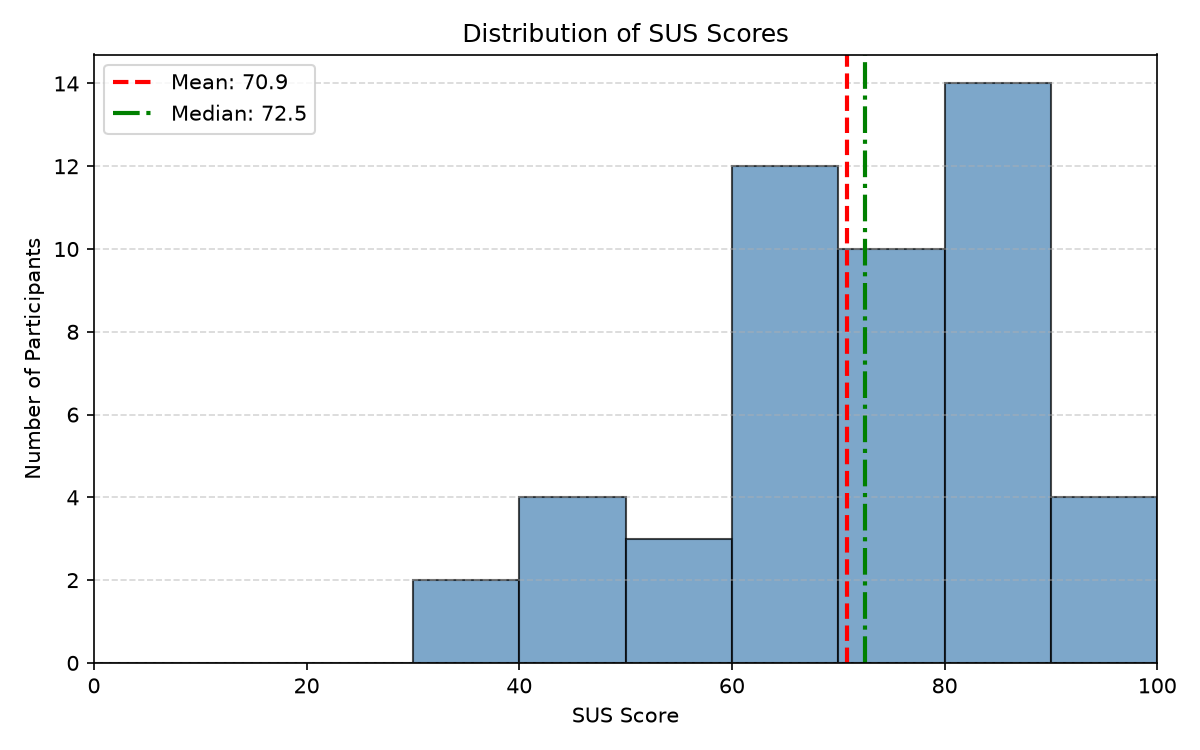
\includegraphics[width=1\linewidth]{sus_histogram.png}
    \caption{SUS Histogram showing the final score distribution over all 49 users that tested the deployed application.}
    \label{fig:sush}
\end{figure}

The results from the System Usability Scale (SUS) questionnaire, collected from the 49 participants who tested the deployed application, provide a strong quantitative validation of our prototype. As depicted in the distribution of SUS scores (visualized in \autoref{fig:sush}), the application achieved a mean SUS score of 70.9 and a median score of 72.5. 

In the standard context of the System Usability Scale, a score of 68 is generally considered the industry average. Our prototype's mean score of 70.9 places its usability comfortably above average, categorizing the overall user experience as ``Good''. The median score of 72.5 further emphasizes this positive reception, demonstrating that more than half of the participants evaluated the system highly. 

Analyzing the distribution of the data, it is evident that the vast majority of users scored the application between 60 and 100. The most frequent scores fell into the 80 to 90 range, which included 14 participants. This strong concentration of high scores indicates that our primary design decisions, such as the simplified, wizard-based ticket selection and the compact route overviews, effectively reduced cognitive load and successfully addressed the initial pain points identified during our insight-gathering phase.

While the overall results firmly validate our approach and confirm that the prototype assists newcomers in navigating Oldenburg's public transport, a small cluster of lower scores (specifically between 30 and 50) highlights room for future refinement. These lower scores likely correspond to specific user edge cases or technical limitations of the prototype (such as static ticket pricing or limited routing data) rather than a failure of the core concept. Ultimately, achieving a 70.9 SUS score confirms that our interaction design cycle successfully produced an accessible and user-friendly solution for our target group.

\subsection{Conclusion}
In conclusion, this project successfully applied the Interaction Design Cycle to address the specific challenges faced by newcomers using public transport in Oldenburg. By gathering user insights through surveys and inquiries, we identified key pain points, such as ticket complexity and routing confusion. The resulting prototype prioritized clarity, accessibility, and a guided ticket selection process over an overwhelming feature set. The quantitative evaluation yielded an above average SUS score, confirming that the design interventions effectively improved usability. While the prototype remains conceptual and is bound by specific technical limitations, it clearly demonstrates that a user-centric interface can significantly lower the barrier to entry for public transport systems.

\subsection{Future Work}
The evaluation and identified technical limitations point to several areas for future work. The most critical step would be the integration of a fully functional live ticket purchasing system, which requires technical and legal collaboration with official transport providers. Additionally, replacing the static pricing and simplified route estimations with a dynamic, real-time routing engine would ensure absolute accuracy for users. Future iterations should also move beyond conceptual designs and fully implement the proposed accessibility features, such as the direct notification system for bus drivers, to evaluate their real-world impact. Finally, expanding the application's scope to include regional travel outside of Oldenburg would provide a more comprehensive and robust mobility solution.



\newpage




% ----------------------------
% Appendices
% ----------------------------
\appendix
\section{Survey Data Structure}
Sample structure of the JSON data collected during the field surveys.

\begin{lstlisting}[language=json, caption={Sample Survey Data Structure}]
{
    "respondent_id": 1,
    "user_type": "newcomer",
    "difficulties": ["routing", "buying tickets"],
    "usage_frequency": "daily"
}
\end{lstlisting}

\begin{figure}[h!]
    \centering
    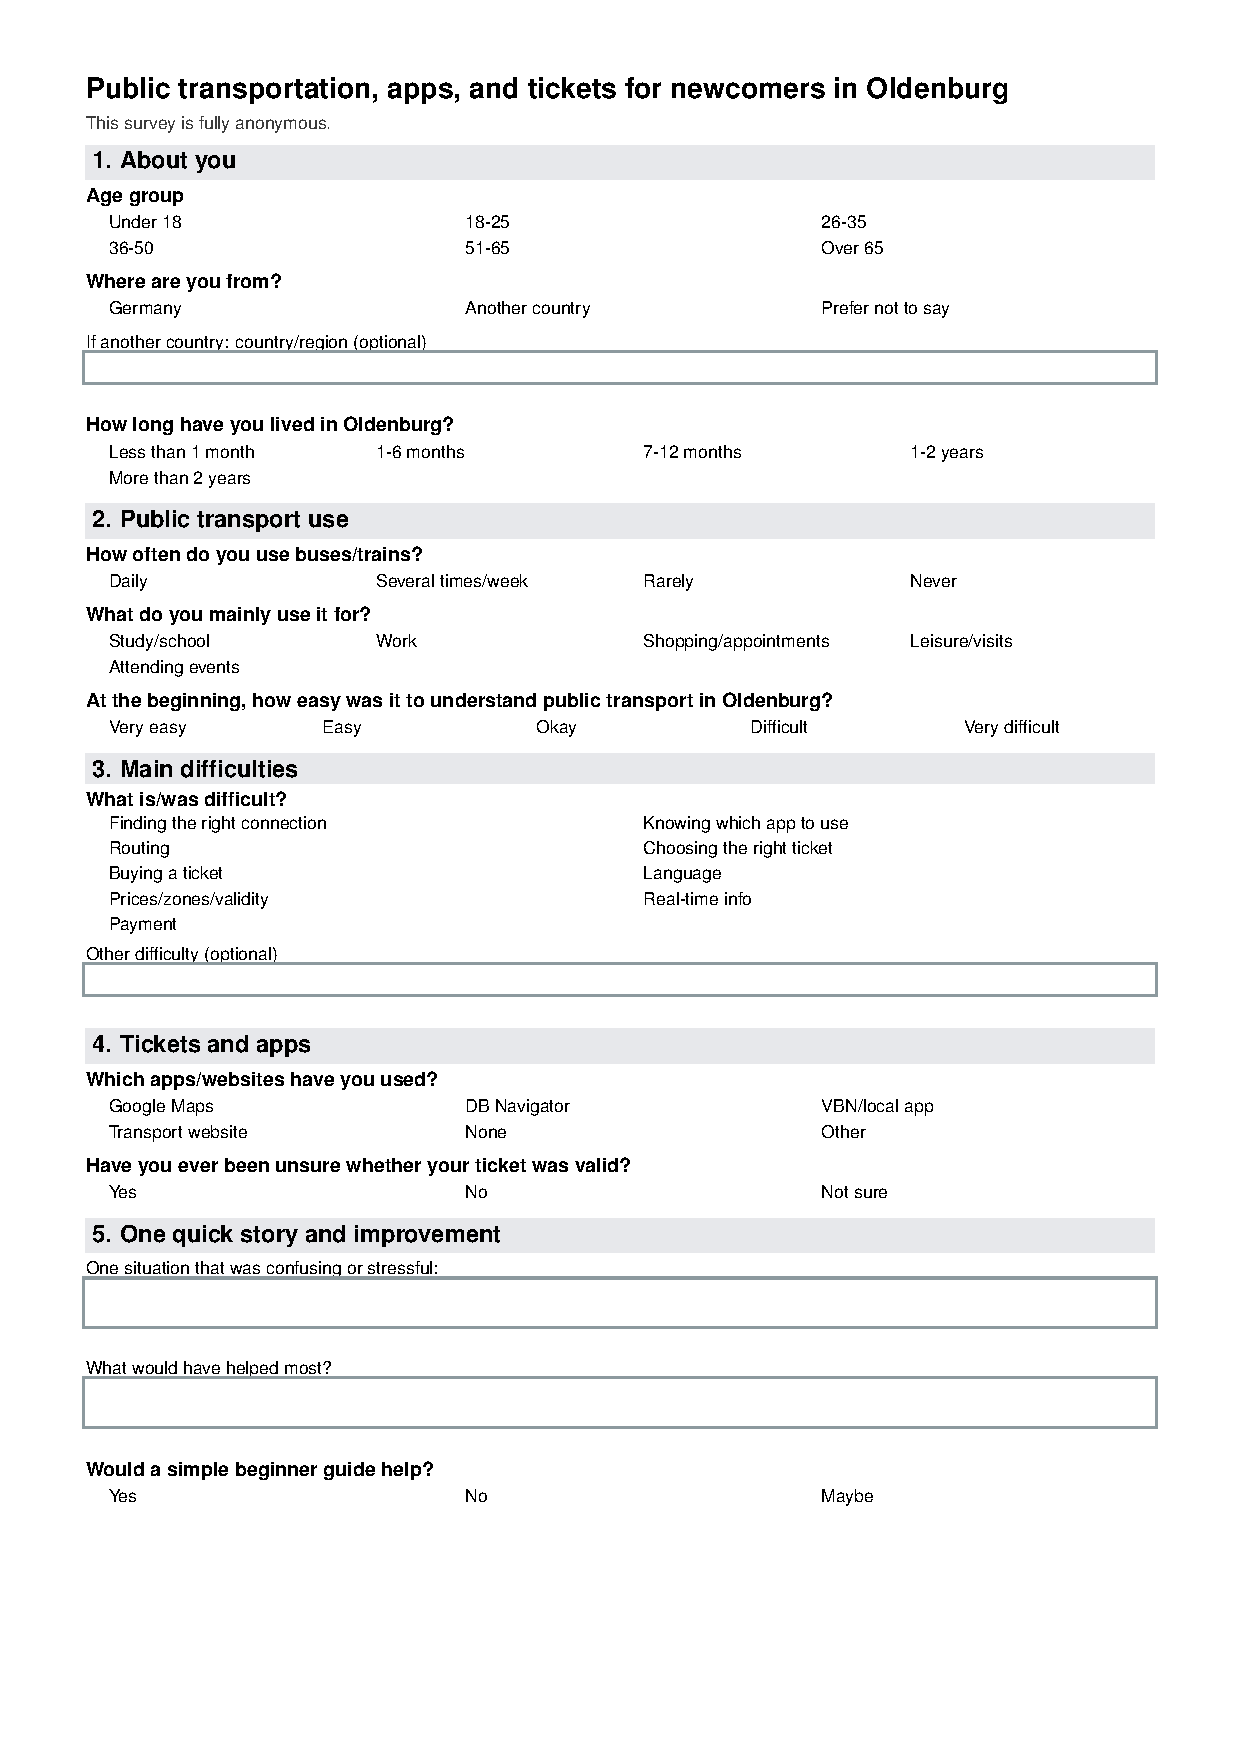
\includegraphics[width=1\linewidth]{interview_sheet.pdf}
    \caption{Survey and interview sheet used for inquiries.}
    \label{fig:inteviewsheet}
\end{figure}

\clearpage

\begin{center}
    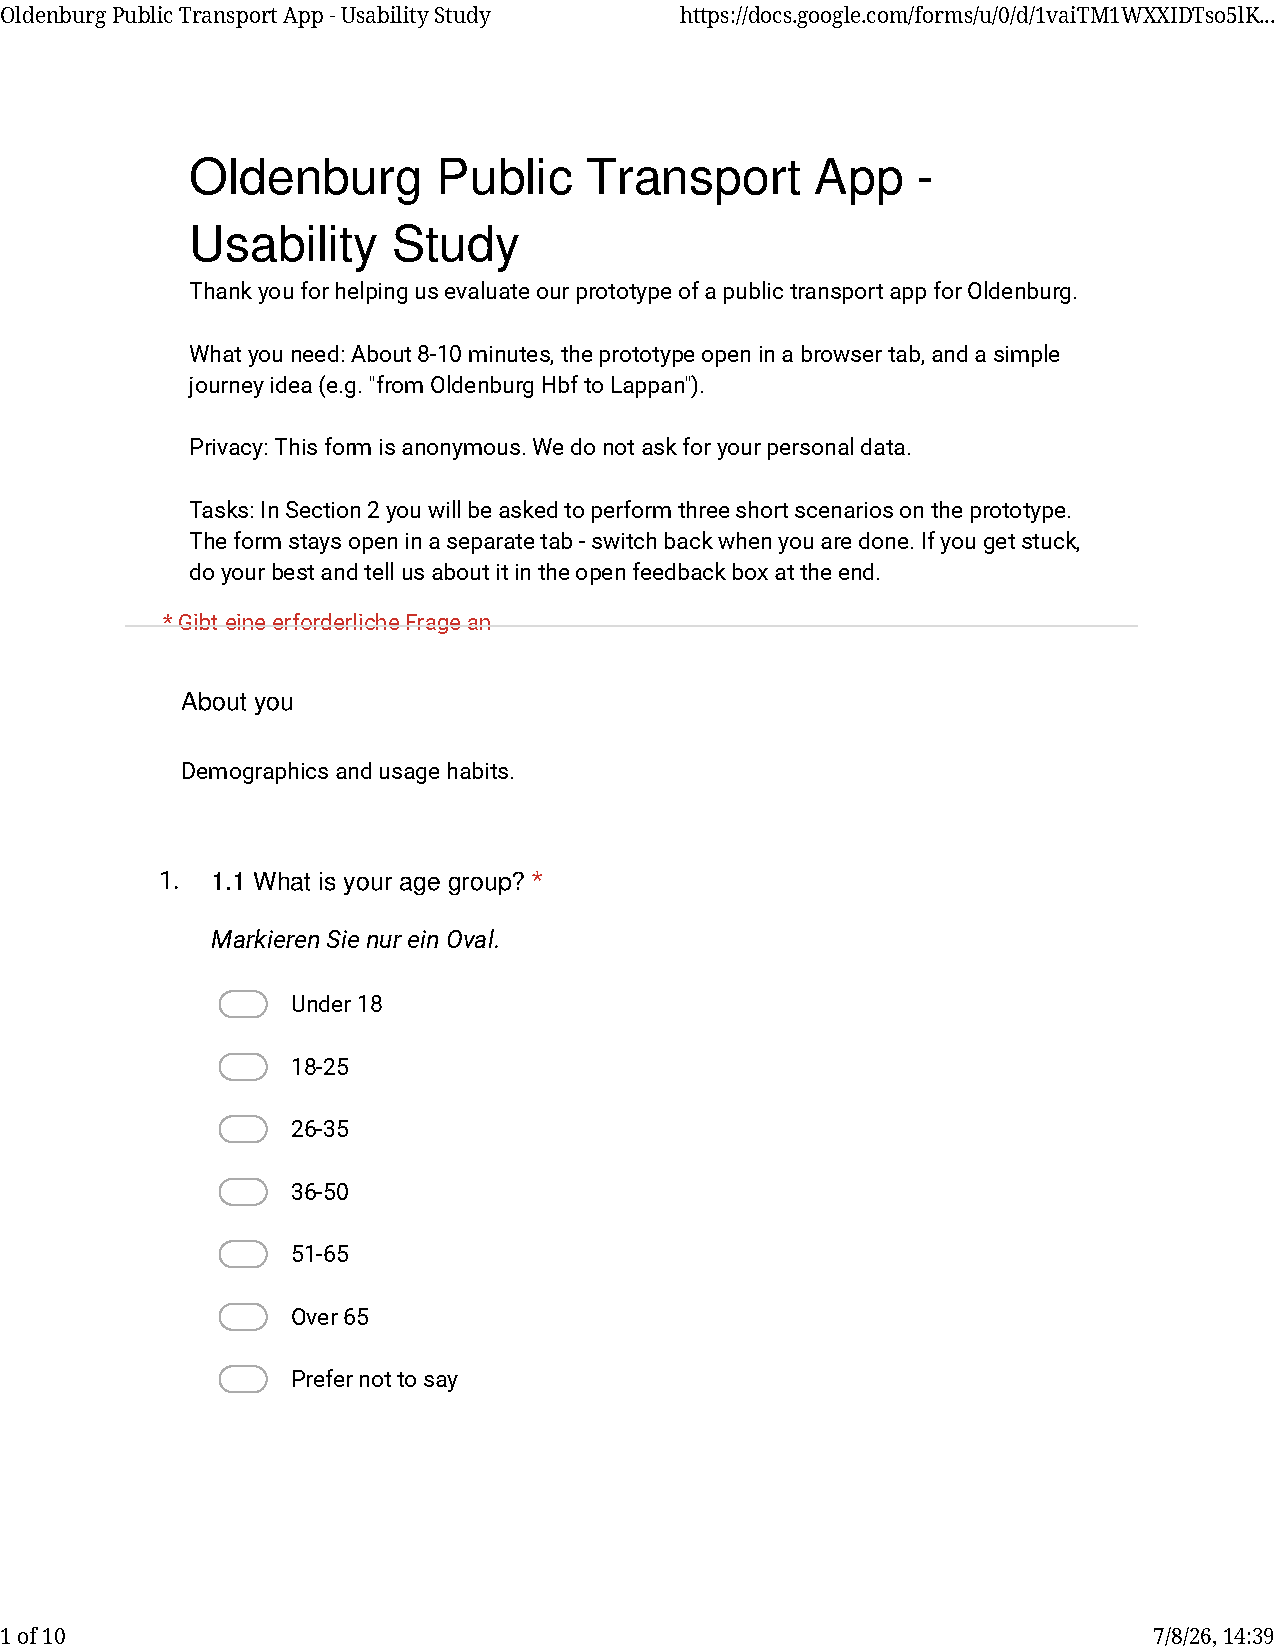
\includegraphics[page=1,width=0.85\linewidth]{Usability_Study.pdf}
    \captionof{figure}{Complete Google Forms questionnaire used for the usability study and gathering user feedback.}
    \label{fig:googleFormsSheet}
\end{center}

\clearpage
\begin{center}\includegraphics[page=2,width=0.85\linewidth]{Usability_Study.pdf}\end{center}

\clearpage
\begin{center}\includegraphics[page=3,width=0.85\linewidth]{Usability_Study.pdf}\end{center}

\clearpage
\begin{center}\includegraphics[page=4,width=0.85\linewidth]{Usability_Study.pdf}\end{center}

\clearpage
\begin{center}\includegraphics[page=5,width=0.85\linewidth]{Usability_Study.pdf}\end{center}

\clearpage
\begin{center}\includegraphics[page=6,width=0.85\linewidth]{Usability_Study.pdf}\end{center}

\clearpage
\begin{center}\includegraphics[page=7,width=0.85\linewidth]{Usability_Study.pdf}\end{center}

\clearpage
\begin{center}\includegraphics[page=8,width=0.85\linewidth]{Usability_Study.pdf}\end{center}

\clearpage
\begin{center}\includegraphics[page=9,width=0.85\linewidth]{Usability_Study.pdf}\end{center}

\clearpage
\begin{center}\includegraphics[page=10,width=0.85\linewidth]{Usability_Study.pdf}\end{center}

\clearpage


\bibliographystyle{plain}
\bibliography{literature}

\end{document}